%%%%%%%%%%%%%%%%%%%%%%%%%%%%%%%%%%%%%%%%%%%%%%%%%%%%%%%%%%%%%%%
%
% Welcome to writeLaTeX --- just edit your LaTeX on the left,
% and we'll compile it for you on the right. If you give
% someone the link to this page, they can edit at the same
% time. See the help menu above for more info. Enjoy!
%
%%%%%%%%%%%%%%%%%%%%%%%%%%%%%%%%%%%%%%%%%%%%%%%%%%%%%%%%%%%%%%%

% --------------------------------------------------------------
% This is all preamble stuff that you don't have to worry about.
% Head down to where it says "Start here"
% --------------------------------------------------------------
 
\documentclass[12pt]{article}
 
\usepackage[margin=1in]{geometry}
\usepackage{amsmath,amsthm,amssymb}
\usepackage{enumitem}
\usepackage{cancel}

\setlist[enumerate,1]{label={(\alph*)}} %this changes enumerate to (a),(b),...

\usepackage{graphicx} %package to manage images

\newcommand{\A}{{\mathcal{A}}}
\newcommand{\C}{{\mathbb C}}
\newcommand{\CC}{{\mathcal{C}}}
\newcommand{\N}{{\mathbb N}}
\newcommand{\R}{{\mathbb R}}
\newcommand{\Q}{{\mathbb Q}}
\newcommand{\Z}{{\mathbb Z}}

\newcommand{\Aut}{{\rm Aut}}
\newcommand{\End}{{\rm End}}
\newcommand{\Hom}{{\rm Hom}}
\newcommand{\id}{{\rm id}}
\newcommand{\Ima}{{\rm Im}}
\newcommand{\Ker}{{\rm Ker}}
\newcommand{\Mor}{{\rm Mor}}
\newcommand{\Rad}{{\rm Rad}}
\newcommand{\Prob}{{\sf P}}
\newcommand{\E}{{\sf E}}
\newcommand{\Var}{{\sf Var}}
\newcommand{\Cov}{{\sf Cov}}
\newcommand{\Corr}{{\sf Corr}}

\renewcommand\labelitemi{-} %this changes itemize bullet points to dashes (-)

\usepackage{listings}
\usepackage{xcolor}

%New colors defined below
\definecolor{codegreen}{rgb}{0,0.6,0}
\definecolor{codegray}{rgb}{0.5,0.5,0.5}
\definecolor{codepurple}{rgb}{0.58,0,0.82}
\definecolor{backcolour}{rgb}{0.95,0.95,0.92}

%Code listing style named "mystyle"
\lstdefinestyle{mystyle}{
  backgroundcolor=\color{backcolour}, commentstyle=\color{codegreen},
  keywordstyle=\color{magenta},
  numberstyle=\tiny\color{codegray},
  stringstyle=\color{codepurple},
  basicstyle=\ttfamily\footnotesize,
  breakatwhitespace=false,         
  breaklines=true,                 
  captionpos=b,                    
  keepspaces=true,                 
  numbers=left,                    
  numbersep=5pt,                  
  showspaces=false,                
  showstringspaces=false,
  showtabs=false,                  
  tabsize=2
}

%"mystyle" code listing set
\lstset{style=mystyle}
 
\newenvironment{theorem}[2][Theorem]{\begin{trivlist}
\item[\hskip \labelsep {\bfseries #1}\hskip \labelsep {\bfseries #2.}]}
{\end{trivlist}}
\newenvironment{lemma}[2][Lemma]{\begin{trivlist}
\item[\hskip \labelsep {\bfseries #1}\hskip \labelsep {\bfseries #2.}]}
{\end{trivlist}}
\newenvironment{exercise}[2][Exercise]{\begin{trivlist}
\item[\hskip \labelsep {\bfseries #1}\hskip \labelsep {\bfseries #2.}]}
{\end{trivlist}}
\newenvironment{problem}[2][Problem]{\begin{trivlist}
\item[\hskip \labelsep {\bfseries #1}\hskip \labelsep {\bfseries #2.}]}
{\end{trivlist}}
\newenvironment{question}[2][Question]{\begin{trivlist}
\item[\hskip \labelsep {\bfseries #1}\hskip \labelsep {\bfseries #2.}]}
{\end{trivlist}}
\newenvironment{corollary}[2][Corollary]{\begin{trivlist}
\item[\hskip \labelsep {\bfseries #1}\hskip \labelsep {\bfseries #2.}]}
{\end{trivlist}}

\newenvironment{solution}{\begin{proof}[Solution]}{\end{proof}}
 
\begin{document}
 
% --------------------------------------------------------------
%                         Start here
% --------------------------------------------------------------
 
\title{Homework 8}%replace X with the appropriate number
\author{Mengxiang Jiang\\ %replace with your name
Stat 610 Distribution Theory} %if necessary, replace with your course title
 
\maketitle

\begin{problem}{1}
  Let $X$ and $Y$ be independent random variables with the \textit{same}
  cdf $F(x)$. Define $U = \min(X,Y)$ and $V = \max(X,Y)$.
  \begin{enumerate}
    \item Show that $\Prob(u < U \le V \le v) = [F(v) - F(u)]^2$, if
    $u < v$. Hint: think about the event in terms of the values of $X$ and $Y$.
    \item Explain why $\Prob(U \le u, V \le v) = \Prob(V \le v) 
    - \Prob(u < U \le V \le v)$, and then deduce the joint cdf for $(U, V )$.
    \item What are the marginal cdfs?
    \item Now assume $F(x)$ has pdf $f(x)$. What are the joint and marginal 
    pdfs for $(U, V )$?
  \end{enumerate}
  \begin{enumerate}
    \item We have
    \begin{align*}
      \Prob(u < U \le V \le v) &= \Prob(u < \min(X,Y) \le \max(X,Y) \le v) \\
      &= \Prob(u < X \le v, u < Y \le v) \\
      &= \Prob(u < X \le v) \cdot \Prob(u < Y \le v) \\
      &= [F(v) - F(u)] \cdot [F(v) - F(u)] \\
      &= [F(v) - F(u)]^2.
  \end{align*}
    \item We have
    \begin{align*}
      \Prob(U \le u, V \le v) &= \Prob(\min(X,Y) \le u, \max(X,Y) \le v) \\
      &= \Prob(X \le v, Y \le v) - \Prob(u < \min(X,Y) \le \max(X,Y) \le v) \\
      &= F(v)^2 - [F(v) - F(u)]^2.
    \end{align*}
    Thus the joint cdf of $(U,V)$ is
    \[
      F_{U,V}(u,v) = \Prob(U \le u, V \le v) = F(v)^2 - (F(v) - F(u))^2.
    \]
    \item The marginal cdf of $U$ is
    \begin{align*}
      F_U(u) &= \Prob(U \le u) = \lim_{v \to \infty} F_{U,V}(u,v) \\
      &= \lim_{v \to \infty} [F(v)^2 - (F(v) - F(u))^2] \\
      &= 1 - (1 - F(u))^2 = 2F(u) - F(u)^2.
    \end{align*}
    The marginal cdf of $V$ is
    \begin{align*}
      F_V(v) &= \Prob(V \le v) = \lim_{u \to -\infty} F_{U,V}(u,v) \\
      &= \lim_{u \to -\infty} [F(v)^2 - (F(v) - F(u))^2] \\
      &= F(v)^2 - (F(v) - 0)^2 = F(v)^2.
    \end{align*}
    \item The joint pdf of $(U,V)$ is
    \[
      f_{U,V}(u,v) = \frac{\partial^2}{\partial u \partial v} 
      [F(v)^2 - (F(v) - F(u))^2] = 2 f(u) f(v).
    \]
    The marginal pdf of $U$ is
    \[
      f_U(u) = \frac{d}{du} [2F(u) - F(u)^2] = 2(1 - F(u)) f(u).
    \]
    The marginal pdf of $V$ is
    \[
      f_V(v) = \frac{d}{dv} [F(v)^2] = 2 F(v) f(v).
    \]
  \end{enumerate}
\end{problem}

\begin{problem}{2}
  Suppose $R \sim \text{exponential}(2)$ (same as chi-square(2)) 
  and $\Theta \sim \text{uniform}(-\pi, \pi)$, independent.
  \begin{enumerate}
    \item Find the joint pdf for $(X_1, X_2) = (R \sin(\Theta), 
    R \cos(\Theta))$. (This is a 1-1 transformation.)
    \item Are $X_1$ and $X_2$ dependent or independent? 
    What are their marginal distributions?
  \end{enumerate}
  \begin{enumerate}
    \item The joint pdf of $(R, \Theta)$ is
    \[
      f_{R, \Theta}(r, \theta) = f_R(r) f_\Theta(\theta) 
      = \frac{1}{2} e^{-\frac{1}{2}r} \cdot \frac{1}{2\pi} 
      = \frac{1}{4\pi} e^{-\frac{1}{2}r},
    \]
    for $r > 0$ and $-\pi < \theta < \pi$. The transformation is
    \[
      g(r, \theta) = (r \sin(\theta), r \cos(\theta)) = (x_1, x_2).
    \]
    The inverse transformation is
    \[
      g^{-1}(x_1, x_2) = (r, \theta) = \left(\sqrt{x_1^2 + x_2^2}, 
      \tan^{-1}\left(\frac{x_1}{x_2}\right)\right).
    \]
    The Jacobian determinant is
    \[
      J = \begin{vmatrix}
        \sin(\theta) & r \cos(\theta) \\
        \cos(\theta) & -r \sin(\theta)
      \end{vmatrix} = -r(\sin^2(\theta) + \cos^2(\theta)) = -r.
    \]
    Thus the joint pdf of $(X_1, X_2)$ is
    \begin{align*}
      f_{X_1, X_2}(x_1, x_2) &= f_{R, \Theta}(g^{-1}(x_1, x_2)) 
      \cdot |J| \\
      &= \frac{1}{4\pi} e^{-\frac{1}{2}\sqrt{x_1^2 + x_2^2}} 
      \cdot \sqrt{x_1^2 + x_2^2} \\
      &= \frac{\sqrt{x_1^2 + x_2^2}}{4\pi} 
      e^{-\frac{1}{2}\sqrt{x_1^2 + x_2^2}},
    \end{align*}
    for $-\infty < x_1, x_2 < \infty$.
    \item The joint pdf $f_{X_1, X_2}(x_1, x_2)$ cannot be factored into
    the product of two functions of $x_1$ and $x_2$ separately, 
    so $X_1$ and $X_2$ are dependent. The marginal pdf of $X_1$ is
    \begin{align*}
      f_{X_1}(x_1) &= \int_{-\infty}^\infty f_{X_1, X_2}(x_1, x_2) \, dx_2 \\
      &= \int_{-\infty}^\infty \frac{\sqrt{x_1^2 + x_2^2}}{4\pi} 
      e^{-\frac{1}{2}\sqrt{x_1^2 + x_2^2}} \, dx_2
    \end{align*}
    Apparently this can be simplified by using Bessel functions, but we
    did not cover that in class. Similarly, the marginal pdf of $X_2$ is
    \begin{align*}
      f_{X_2}(x_2) &= \int_{-\infty}^\infty f_{X_1, X_2}(x_1, x_2) \, dx_1 \\
      &= \int_{-\infty}^\infty \frac{\sqrt{x_1^2 + x_2^2}}{4\pi} 
      e^{-\frac{1}{2}\sqrt{x_1^2 + x_2^2}} \, dx_1.
    \end{align*}
  \end{enumerate}
\end{problem}

\begin{problem}{3}
  Recall Problem 6 of Assignment 7, where $(R, S)$ has joint 
  pdf $f_{R,S} (r, s) = \frac{8}{3} s^2 e^{-2s}$ for
  $0 \le r \le s$. You may use the solutions from that problem.
  \begin{enumerate}
    \item Find the mean and variance of $S$.
    \item Find $\E(R|S = s)$ and $\E(R^2|S = s)$. Then use iterated 
    expectation and the variance partition formula to compute the 
    mean and variance of $R$.
    \item Use iterated expectation to find $\E(RS) = \E(\E(RS|S))$.
    \item Now use the above to determine $\Cov(R, S)$.
  \end{enumerate}

  \begin{enumerate}
    \item From the solution of Problem 6 of Assignment 7,
    we know that $S$ follows a gamma distribution with parameters
    $\alpha = 4$ and $\beta = \frac{1}{2}$. Since the mean and variance
    of a gamma distribution are
    $\alpha \beta$ and $\alpha \beta^2$, respectively, we have
    \[
      \E(S) = 4 \cdot \frac{1}{2} = 2, \quad \Var(S) = 4 \cdot 
      \left(\frac{1}{2}\right)^2 = 1.
    \]
    \item We have
    \[
      f_{R|S}(r|s) = \frac{f_{R,S}(r,s)}{f_S(s)} 
      = \frac{\frac{8}{3} s^2 e^{-2s}}{\frac{8}{3} s^3 e^{-2s}} = \frac{1}{s},
    \]
    for $0 \le r \le s$. Thus
    \[
      \E(R|S = s) = \int_0^s r \cdot \frac{1}{s} \, dr 
      = \frac{s}{2},
    \]
    and
    \[
      \E(R^2|S = s) = \int_0^s r^2 \cdot \frac{1}{s} \, dr 
      = \frac{s^2}{3}.
    \]
    By iterated expectation, we have
    \[
      \E(R) = \E(\E(R|S)) = \E\left(\frac{S}{2}\right) 
      = \frac{1}{2} \E(S) = 1.
    \]
    By the variance partition formula, we have
    \begin{align*}
      \Var(R) &= \E(\Var(R|S)) + \Var(\E(R|S)) \\
      &= \E\left(\E(R^2|S) - (\E(R|S))^2\right) 
      + \Var\left(\frac{S}{2}\right) \\
      &= \E\left(\frac{S^2}{3} - \left(\frac{S}{2}\right)^2\right) 
      + \frac{1}{4} \Var(S) \\
      &= \E\left(\frac{S^2}{3} - \frac{S^2}{4}\right) + \frac{1}{4} \\
      &= \E\left(\frac{S^2}{12}\right) + \frac{1}{4} \\
      &= \frac{1}{12} \E(S^2) + \frac{1}{4}.
    \end{align*}
    Since $\Var(S) = \E(S^2) - (\E(S))^2$, we have
    \[
      \E(S^2) = \Var(S) + (\E(S))^2 = 1 + 2^2 = 5.
    \]
    Thus
    \[
      \Var(R) = \frac{1}{12} \cdot 5 + \frac{1}{4} = \frac{5}{12} + 
      \frac{3}{12} = \frac{8}{12} = \frac{2}{3}.
    \]
    \item By iterated expectation, we have
    \[
      \E(RS) = \E(\E(RS|S)) = \E\left(S \cdot \E(R|S)\right) 
      = \E\left(S \cdot \frac{S}{2}\right) = \frac{1}{2} \E(S^2) 
      = \frac{1}{2} \cdot 5 = \frac{5}{2}.
    \]
    \item We have
    \[
      \Cov(R, S) = \E(RS) - \E(R)\E(S) = \frac{5}{2} - 1 \cdot 2 = 
      \frac{5}{2} - 2 = \frac{1}{2}.
    \]
  \end{enumerate}
\end{problem}

\begin{problem}{4} 
  Suppose $W \sim \text{Poisson}(\lambda)$ and the conditional distribution 
  of $X$, given $W = w$, is exponential($w^2$) if $w > 0$ and 
  $X = 0$ if $w = 0$. So, in particular, $\E(X|W ) = W^2$.\\
  Find the mean and variance of $X$. You may use (without proof) the 
  following fact:
  \[
    \E(W (W - 1) \times \cdots \times (W - k)) = \lambda^{k+1}, 
    \quad k = 1, 2, \dots
  \]
  Since $W$ is Poisson, its mean and variance are both $\lambda$.
  Since the conditional distribution of $X$ given $W = w$ is 
  exponential($w^2$) for $w > 0$, we have
  \[
    \E(X|W = w) = w^2, \quad \Var(X|W = w) = w^4.
  \]
  Thus,
  \begin{align*}
    \E(X) &= \E(\E(X|W)) = \E(W^2) \\
    &= \Var(W) + (\E(W))^2 = \lambda + \lambda^2.
  \end{align*}
  By the variance partition formula, we have
  \begin{align*}
    \Var(X) &= \E(\Var(X|W)) + \Var(\E(X|W)) \\
    &= \E(W^4) + \Var(W^2).
  \end{align*}
  We can express $W^4$ in terms of falling factorials as
  \[
    W^4 = W (W - 1) (W - 2) (W - 3) + 6 W (W - 1) (W - 2) 
    + 7 W (W - 1) + W.
  \]
  Thus,
  \begin{align*}
    \E(W^4) &= \E(W (W - 1) (W - 2) (W - 3)) + 6 \E(W (W - 1) (W - 2)) \\
    &\quad + 7 \E(W (W - 1)) + \E(W) \\
    &= \lambda^4 + 6 \lambda^3 + 7 \lambda^2 + \lambda.
  \end{align*}
  Next, we compute $\Var(W^2)$ as
  \begin{align*}
    \Var(W^2) &= \E(W^4) - (\E(W^2))^2 \\
    &= (\lambda^4 + 6 \lambda^3 + 7 \lambda^2 + \lambda) 
    - (\lambda + \lambda^2)^2 \\
    &= (\lambda^4 + 6 \lambda^3 + 7 \lambda^2 + \lambda) 
    - (\lambda^4 + 2 \lambda^3 + \lambda^2) \\
    &= 4 \lambda^3 + 6 \lambda^2 + \lambda.
  \end{align*}
  Therefore, we have
  \begin{align*}
    \Var(X) &= \E(W^4) + \Var(W^2) \\
    &= (\lambda^4 + 6 \lambda^3 + 7 \lambda^2 + \lambda) 
    + (4 \lambda^3 + 6 \lambda^2 + \lambda) \\
    &= \lambda^4 + 10 \lambda^3 + 13 \lambda^2 + 2 \lambda.
  \end{align*}
\end{problem}

\begin{problem}{5}
  Recall Exercise 4.4 (Problem 5 of Assignment 7):\\
  A pdf is defined by
    \[
      f(x,y) = \begin{cases}
        C(x+2y) & \text{if } 0 < y < 1 \text{ and } 0 < x < 2 \\
        0 & \text{otherwise.}
      \end{cases}
    \]
  where $C = \frac{1}{4}$.
  Now do the following.
  \begin{enumerate}
    \item Determine the conditional pdf for $Y$, given $X = x$, 
    and the conditional pdf for $X$, given
    $Y = y$.
    \item Find $g(x) = \E(Y |X = x)$ and $h(y) = \E(X|Y = y)$. Are either of
    these linear? Are they inverses of each other?
    \item Plot $y = g(x)$ versus $x$ and $y$ versus $x = h(y)$ on 
    the same graph. Comment on what they indicate about predicting 
    one random variable from the other.
    \item Compute $\E(X)$, $\E(Y )$ and $\E(XY )$ by whatever
    method(s) you prefer.
    \item Compute $\Cov(X, Y )$.
  \end{enumerate}
  \begin{enumerate}
    \item The marginal pdf of $X$ is
    \begin{align*}
      f_X(x) &= \int_0^1 f(x,y) \, dy \\
      &= \int_0^1 C(x + 2y) \, dy = C \left(x + 1\right),
    \end{align*}
    for $0 < x < 2$. The marginal pdf of $Y$ is
    \begin{align*}
      f_Y(y) &= \int_0^2 f(x,y) \, dx \\
      &= \int_0^2 C(x + 2y) \, dx = C \left(1 + 4y\right),
    \end{align*}
    for $0 < y < 1$. Thus the conditional pdf of $Y$ given $X = x$ is
    \begin{align*}
      f_{Y|X}(y|x) &= \frac{f(x,y)}{f_X(x)} = \frac{C(x + 2y)}{C(x + 1)} 
      = \frac{x + 2y}{x + 1}, \quad 0 < y < 1.
    \end{align*}
    The conditional pdf of $X$ given $Y = y$ is
    \begin{align*}
      f_{X|Y}(x|y) &= \frac{f(x,y)}{f_Y(y)} = \frac{C(x + 2y)}{C(1 + 4y)} \\
      &= \frac{x + 2y}{1 + 4y}, \quad 0 < x < 2.
    \end{align*}
    \item We have
    \begin{align*}
      g(x) = \E(Y|X = x) &= \int_0^1 y \cdot \frac{x + 2y}{x + 1} \, dy \\
      &= \frac{1}{x + 1} \int_0^1 (xy + 2y^2) \, dy \\
      &= \frac{1}{x + 1} \left(\frac{x}{2} + \frac{2}{3}\right) 
      = \frac{3x + 4}{6(x + 1)}.
    \end{align*}
    Similarly,
    \begin{align*}
      h(y) = \E(X|Y = y) &= \int_0^2 x \cdot \frac{x + 2y}{1 + 4y} \, dx \\
      &= \frac{1}{1 + 4y} \int_0^2 (x^2 + 2yx) \, dx \\
      &= \frac{1}{1 + 4y} \left(\frac{8}{3} + 4y\right) 
      = \frac{8 + 12y}{3(1 + 4y)}.
    \end{align*}
    Neither $g(x)$ nor $h(y)$ is linear. They are not inverses of each other
    since $g(h(y)) \neq y$ and $h(g(x)) \neq x$.
    \item The plot is shown below.
    \begin{center}
      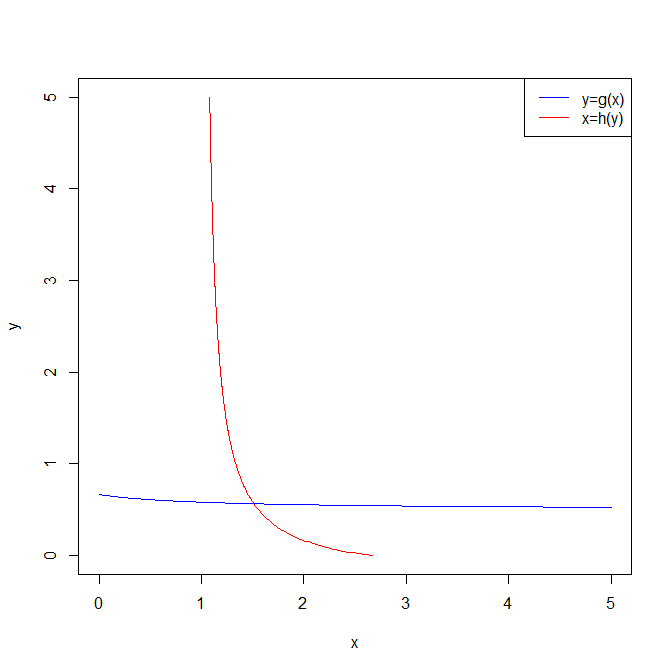
\includegraphics[width=0.8\textwidth]{5c.png}
    \end{center}
    From the plot, we can see that both $g(x)$ and $h(y)$ are decreasing
    functions. This indicates that when predicting $Y$ from $X$, a larger
    value of $X$ tends to correspond to a smaller predicted value of $Y$,
    and vice versa.
    \item
    \begin{align*}
      \E(X) &= \int_0^2 x f_X(x) \, dx = \int_0^2 x C(x + 1) \, dx 
      = C \int_0^2 (x^2 + x) \, dx = C \left(\frac{8}{3} + 2\right) 
      = \frac{7}{6}, \\
      \E(Y) &= \int_0^1 y f_Y(y) \, dy = \int_0^1 y C(1 + 4y) \, dy 
      = C \int_0^1 (y + 4y^2) \, dy = C \left(\frac{1}{2} + \frac{4}{3}\right) 
      = \frac{7}{12},\\
      \E(XY) &= \int_0^2 \int_0^1 xy f(x,y) \, dy \, dx \\
      &= \int_0^2 \int_0^1 xy C(x + 2y) \, dy \, dx \\
      &= C \int_0^2 \left( x^2 \int_0^1 y \, dy + 2x \int_0^1 y^2 \, dy \right) dx \\
      &= C \int_0^2 \left( x^2 \cdot \frac{1}{2} + 2x \cdot \frac{1}{3} \right) dx \\
      &= C \int_0^2 \left( \frac{x^2}{2} + \frac{2x}{3} \right) dx \\
      &= C \left( \frac{8}{6} + \frac{4}{3} \right) = C \cdot \frac{16}{6} \\
      &= \frac{2}{3}.
    \end{align*}
    \item
    \begin{align*}
      \Cov(X, Y) &= \E(XY) - \E(X) \E(Y) \\
      &= \frac{2}{3} - \frac{7}{6} \cdot \frac{7}{12} \\
      &= \frac{2}{3} - \frac{49}{72} = \frac{48}{72} - \frac{49}{72} 
      = -\frac{1}{72}.
    \end{align*}
  \end{enumerate}
\end{problem}

\begin{problem}{6}
  Assume the random pair $(S, T )$ has joint distribution
  \[
  f_{S,T}(s, t) = \frac{1}{2} (s + t)e^{-(s+t)}, \quad s > 0, t > 0.
  \]
  \begin{enumerate}
    \item Find $\E(S)$, $\E(S^2)$, $\E(T)$, $\E(T^2)$ and $\E(ST)$. 
    Hint: you can express each of these in terms of some gamma function values.
    \item Determine $\Corr(S, T)$.
  \end{enumerate}
  \begin{enumerate}
    \item We have
    \begin{align*}
      \E(S) &= \int_0^\infty \int_0^\infty s \cdot \frac{1}{2} (s + t) 
      e^{-(s+t)} \, dt \, ds \\
      &= \frac{1}{2} \int_0^\infty s e^{-s} \left( \int_0^\infty (s + t) 
      e^{-t} \, dt \right) ds \\
      &= \frac{1}{2} \int_0^\infty s e^{-s} (s + 1) \, ds \\
      &= \frac{1}{2} (\Gamma(3) + \Gamma(2)) = \frac{1}{2} (2 + 1) = 
      \frac{3}{2}.\\
      \E(S^2) &= \int_0^\infty \int_0^\infty s^2 \cdot \frac{1}{2} (s + t) 
      e^{-(s+t)} \, dt \, ds \\
      &= \frac{1}{2} \int_0^\infty s^2 e^{-s} (s + 1) \, ds \\
      &= \frac{1}{2} (\Gamma(4) + \Gamma(3)) = \frac{1}{2} (6 + 2) = 4, \\
      \text{By symmetry,} \\
      \E(T) &= E[S] = \frac{3}{2}, \\
      \E(T^2) &= E[S^2] = 4.
    \end{align*}
    Using the change of variables $u = s + t$, we have
    \begin{align*}
      \E(ST) &= \frac{1}{2}\int_0^\infty u e^{-u} \int_0^u s (u - s) \, ds \, du \\
      &= \frac{1}{2} \int_0^\infty u e^{-u} \left( \frac{u^3}{6} \right) du \\
      &= \frac{1}{12} \int_0^\infty u^4 e^{-u} \, du\\
      &= \frac{1}{12} \Gamma(5) = \frac{1}{12} \cdot 24 = 2.
    \end{align*}
    \item We have
    \begin{align*}
      \Cov(S, T) &= \E(ST) - \E(S) \E(T) \\
      &= 2 - \frac{3}{2} \cdot \frac{3}{2} = 2 - \frac{9}{4} 
      = -\frac{1}{4}, \\
      \Var(S) &= \E(S^2) - (\E(S))^2 = 4 - \left(\frac{3}{2}\right)^2 
      = 4 - \frac{9}{4} = \frac{7}{4}, \\
      \Var(T) &= \Var(S) = \frac{7}{4}.
    \end{align*}
    Thus, we have
    \begin{align*}
      \Corr(S, T) &= \frac{\Cov(S, T)}{\sqrt{\Var(S) \Var(T)}} \\
      &= \frac{-\frac{1}{4}}{\sqrt{\frac{7}{4} \cdot \frac{7}{4}}} = 
      \frac{-\frac{1}{4}}{\frac{7}{4}} = -\frac{1}{7}.
    \end{align*}
  \end{enumerate}
\end{problem}

\begin{problem}{7}
  Suppose $X$ and $Y$ are \textit{integer-valued} rvs with joint pmf
  \[
    f_{X,Y}(x, y) = \frac{1}{13}, \quad 
    \text{if } |x + y| \leq 2 \text{ and } |x - y| \leq 2.
  \]
  (It may help to graph the possible points $(x, y)$.)
  \begin{enumerate}
    \item Are $X$ and $Y$ independent? What are their marginal pmfs?
    \item What is $\Cov(X, Y)$?
  \end{enumerate}
  \begin{enumerate}
    \item The possible points $(x, y)$ are
    \[
      (-2, 0), (-1, -1), (-1, 0), (-1, 1), (0, -2), (0, -1), (0, 0), 
      (0, 1), (0, 2), (1, -1), (1, 0), (1, 1), (2, 0).
    \]
    Thus, the marginal pmf of $X$ is
    \[
      f_X(x) = \begin{cases}
        \frac{1}{13} & x = -2 \\
        \frac{3}{13} & x = -1 \\
        \frac{5}{13} & x = 0 \\
        \frac{3}{13} & x = 1 \\
        \frac{1}{13} & x = 2 \\
        0 & \text{otherwise.}
      \end{cases}
    \]
    The marginal pmf of $Y$ is $f_Y(y) = f_X(y)$ by symmetry.
    Since $f_{X,Y}(0,0) = \frac{1}{13} \neq f_X(0) f_Y(0) = 
    \frac{5}{13} \cdot \frac{5}{13} = \frac{25}{169}$, $X$ and $Y$ are not independent.
    \item We have
    \begin{align*}
      \E(X) &= \sum_x x f_X(x) = -2 \cdot \frac{1}{13} - 1 \cdot \frac{3}{13} 
      + 0 \cdot \frac{5}{13} + 1 \cdot \frac{3}{13} + 2 \cdot \frac{1}{13} = 0, \\
      \E(Y) &= \E(X) = 0, \\
      \E(XY) &= \sum_x \sum_y xy f_{X,Y}(x,y) \\
      &= (0 + 1 + 0 - 1 + 0 + 0 + 0 + 0 + 0 - 1 + 0 + 1 + 0) 
      \cdot \frac{1}{13} = 0.
    \end{align*}
    Thus, we have
    \begin{align*}
      \Cov(X, Y) &= \E(XY) - \E(X) \E(Y) \\
      &= 0 - 0 \cdot 0 = 0.
    \end{align*}
  \end{enumerate}
\end{problem}

\begin{problem}{8}
  \begin{enumerate}
    \item Use Theorem 4.22 in the notes to prove that if $X_1, \ldots, X_k$ 
    are independent random variables with respective mgfs 
    $M_1(t), \ldots, M_k(t)$ then the mgf for $S = X_1 + \cdots + X_k$ is
    $M_S(t) = \prod_{i=1}^k M_i(t)$.
    \item Use the result in part (a) to confirm the following.
    \begin{itemize}
      \item[i.] If $S \sim \text{binomial}(m, p)$ and 
      $T \sim \text{binomial}(n, p)$, independent, then $S + T \sim
      \text{binomial}(m+n, p)$. (This was done by use of a convolution 
      in Assignment 6 Problem 4.)
      \item[ii.] If $T$ and $U$ are independent with 
      $T \sim \text{gamma}(\alpha, \gamma)$ and 
      $U \sim \text{gamma}(\beta, \gamma)$ then
      $T + U \sim \text{gamma}(\alpha + \beta, \gamma)$. 
      (You also showed this in Assignment 7 Problem 8 using
      a different method.)
      \item[iii.] If $X \sim \text{Poisson}(\lambda)$ and 
      $Y \sim \text{Poisson}(\mu)$, independent, then 
      $X + Y \sim \text{Poisson}(\lambda + \mu)$.
      (This was also done by convolution in Theorem 4.10 of the notes.)
    \end{itemize}
  \end{enumerate}
  \begin{theorem}{4.22}
    Suppose $(X_1, \ldots, X_k)$ has joint distribution. 
    Then $X_1, \ldots, X_k$ are independent if and only if
    \[
      \E(g_1(X_1) \times \cdots \times g_k(X_k)) = 
      \E(g_1(X_1)) \times \cdots \times \E(g_k(X_k))
    \]
    whenever these expectations exist. $(g_1(X_1), \ldots, g_k(X_k))$ 
    are also independent.\\
    In particular, if $X$ and $Y$ are independent
    and have finite means then $\E(XY) = \E(X) \E(Y)$.
  \end{theorem}
  \begin{enumerate}
    \item Since $X_1, \ldots, X_k$ are independent, by Theorem 4.22, we have
    \begin{align*}
      M_S(t) &= \E(e^{tS}) = \E(e^{t(X_1 + \cdots + X_k)}) \\
      &= \E(e^{tX_1} \times \cdots \times e^{tX_k}) \\
      &= \E(e^{tX_1}) \times \cdots \times \E(e^{tX_k}) \\
      &= M_1(t) \times \cdots \times M_k(t) = \prod_{i=1}^k M_i(t).
    \end{align*}
    \item
    \begin{itemize}
      \item[i.] The mgf of $S \sim \text{binomial}(m, p)$ is
      \[
        M_S(t) = (1 - p + p e^t)^m,
      \]
      and the mgf of $T \sim \text{binomial}(n, p)$ is
      \[
        M_T(t) = (1 - p + p e^t)^n.
      \]
      Thus, the mgf of $S + T$ is
      \[
        M_{S+T}(t) = M_S(t) M_T(t) = (1 - p + p e^t)^{m+n},
      \]
      which is the mgf of $\text{binomial}(m+n, p)$.
      \item[ii.] The mgf of $T \sim \text{gamma}(\alpha, \gamma)$ is
      \[
        M_T(t) = (1 - \gamma t)^{-\alpha}, \quad t < \frac{1}{\gamma},
      \]
      and the mgf of $U \sim \text{gamma}(\beta, \gamma)$ is
      \[
        M_U(t) = (1 - \gamma t)^{-\beta}, \quad t < \frac{1}{\gamma}.
      \]
      Thus, the mgf of $T + U$ is
      \[
        M_{T+U}(t) = M_T(t) M_U(t) = (1 - \gamma t)^{-(\alpha + \beta)},
      \]
      which is the mgf of $\text{gamma}(\alpha + \beta, \gamma)$.
      \item[iii.] The mgf of $X \sim \text{Poisson}(\lambda)$ is
      \[
        M_X(t) = e^{\lambda (e^t - 1)},
      \]
      and the mgf of $Y \sim \text{Poisson}(\mu)$ is
      \[
        M_Y(t) = e^{\mu (e^t - 1)}.
      \]
      Thus, the mgf of $X + Y$ is
      \[
        M_{X+Y}(t) = M_X(t) M_Y(t) = e^{(\lambda + \mu) (e^t - 1)},
      \]
      which is the mgf of $\text{Poisson}(\lambda + \mu)$.
    \end{itemize}
  \end{enumerate}
\end{problem}

% --------------------------------------------------------------
%     You don't have to mess with anything below this line.
% --------------------------------------------------------------
\end{document}
